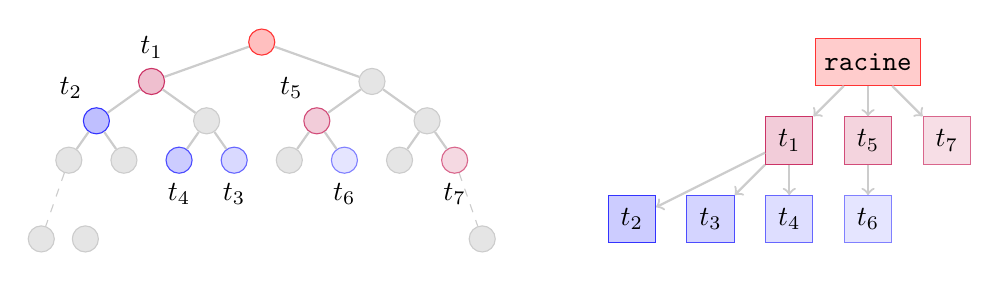
\begin{tikzpicture}
    [   
    cnode/.style={draw=gray!40,fill=gray!20,minimum width=0.2mm,circle},
    colnode/.style={draw=red!80,fill=red!40,minimum width=0.2mm,circle},
    cline/.style={gray!40,thick},
    rnode/.style={draw=gray!40,fill=gray!20,minimum width=6mm, minimum height=6mm, rectangle},
    recnode/.style={fill=#1,minimum width=0.2mm,circle},
    r1node/.style={draw=#1!80,fill=#1!25,minimum width=0.2mm,circle},
    r2node/.style={draw=#1!70,fill=#1!20,minimum width=0.2mm,circle},
    r3node/.style={draw=#1!60,fill=#1!15,minimum width=0.2mm,circle},
    r4node/.style={draw=#1!50,fill=#1!10,minimum width=0.2mm,circle},
    t1node/.style={draw=#1!80,fill=#1!20,minimum width=6mm, minimum height=6mm, rectangle},
    t2node/.style={draw=#1!70,fill=#1!17,minimum width=6mm, minimum height=6mm, rectangle},
    t3node/.style={draw=#1!60,fill=#1!13,minimum width=6mm, minimum height=6mm, rectangle},
    t4node/.style={draw=#1!50,fill=#1!10,minimum width=6mm, minimum height=6mm, rectangle},
    ]
    
    %
    % CLUSTERING TREE
    %
    
    \def\stepx{0.7};
    \def\stepy{0.5};
    
    \node[r3node=blue, label=270:$t_3$] (000) at (-0.5*\stepx,-2*\stepy) {};
    \node[r2node=blue, label=270:$t_4$] (001) at (-1.5*\stepx,-2*\stepy) {};
    \node[cnode] (010) at (-2.5*\stepx,-2*\stepy) {};
    \node[cnode] (011) at (-3.5*\stepx,-2*\stepy) {};
    \node[cnode] (100) at (0.5*\stepx,-2*\stepy) {};
    \node[r4node=blue, label=270:$t_6$] (101) at (1.5*\stepx,-2*\stepy) {};
    \node[cnode] (110) at (2.5*\stepx,-2*\stepy) {};
    \node[r3node=purple, label=270:$t_7$] (111) at (3.5*\stepx,-2*\stepy) {};
    
    \node[r1node=blue, label=110:$t_2$] (00) at (-3*\stepx,-\stepy) {};
    \node[cnode] (01) at (-1*\stepx,-\stepy) {};
    \node[r2node=purple, label=110:$t_5$] (10) at (1*\stepx,-\stepy) {};
    \node[cnode] (11) at (3*\stepx,-\stepy) {};
    
    \node[r1node=purple, label=90:$t_1$] (0) at (-2*\stepx,0*\stepy) {};
    \node[cnode] (1) at (2*\stepx,0*\stepy) {};
    
    \node[r1node=red] (root) at (0,\stepy) {};
    
    
    \def\minx{-5.5*\stepx};
    
    \node[cnode] (t1) at (-4*\stepx,-4*\stepy) {};
    \node[cnode] (t2) at (-3.2*\stepx,-4*\stepy) {};
    \node[cnode] (tn) at (4*\stepx,-4*\stepy) {};
    
    \draw[cline] (root) -- (0) {};
    \draw[cline] (root) -- (1) {};
    
    \draw[cline] (00) -- (0) {};
    \draw[cline] (10) -- (1) {};
    \draw[cline] (01) -- (0) {};
    \draw[cline] (11) -- (1) {};
    
    \draw[cline] (01) -- (000) {};
    \draw[cline] (01) -- (001) {};
    \draw[cline] (00) -- (010) {};
    \draw[cline] (00) -- (011) {};
    \draw[cline] (10) -- (100) {};
    \draw[cline] (10) -- (101) {};
    \draw[cline] (11) -- (110) {};
    \draw[cline] (11) -- (111) {};
    
    \draw[dashed,gray!40] (011) -- (t1) {};
    \draw[dashed,gray!40] (111) -- (tn) {};
    
    %
    % EXTRACTED TAXONOMY
    %
    
    \def\offsety{0.5*\stepy}; %-6*\stepy};
    \def\offsetx{11*\stepx};

    \node[t1node=red] (l11) at (0+\offsetx, \offsety) {\texttt{racine}};
    
    \node[t1node=purple] (l21) at (-1+\offsetx, \offsety-1) {$t_1$};
    \node[t2node=purple] (l22) at (0+\offsetx, \offsety-1) {$t_5$};
    \node[t3node=purple] (l23) at (1+\offsetx, \offsety-1) {$t_7$};
    
    \node[t1node=blue] (l31) at (-3 + \offsetx, \offsety-2) {$t_2$};
    \node[t2node=blue] (l32) at (-2 + \offsetx, \offsety-2) {$t_3$};
    \node[t3node=blue] (l33) at (-1 + \offsetx, \offsety-2) {$t_4$};
    \node[t4node=blue] (l34) at  (0 + \offsetx, \offsety-2) {$t_6$};
    
    \draw[->, gray!40, thick] (l11) -- (l21) {};
    \draw[->, gray!40, thick] (l11) -- (l22) {};
    \draw[->, gray!40, thick] (l11) -- (l23) {};
    \draw[->, gray!40, thick] (l21) -- (l31) {};
    \draw[->, gray!40, thick] (l21) -- (l32) {};
    \draw[->, gray!40, thick] (l21) -- (l33) {};
    \draw[->, gray!40, thick] (l22) -- (l34) {};
\end{tikzpicture}